\chapter{Testing and Plotting}
In this chapter we want to explain how the experiments were conducted and how to interpret the plots what will be used to showcase the results of those experiments in Chapter \ref{experiments_chapter}. We also want to show how to use the testing and plotting systems implemented as part of this project.

\section{Conducting the experiments}
The process of conducting experiments encountered several challenges and fluctuations. the primary concern was to determine the minimum number of rotations (\texttt{rots}) and distances (\texttt{dists}) required to make learning feasible for each obstacle type. After experimenting with up to 30 rotations in some cases, and not getting satisfying results with seemingly any combination of other parameters, it was determined that the game's difficulty in later levels was the root of the problem, as it was impossible to play with some environments(confirmed by human players). Consequently, the game had to be adjusted and thus, there are slight variations in parameters, such as the starting speed and distances between obstacles, in the version of the Space-Run game used in this thesis, as compared to the original. As per a human player's assessment, it is now possible to play all environment combinations until level 15 or even beyond. It is noteworthy that level 10 was the initial choice for the winning level, which was later shifted to level 15 to prevent the agent from settling for a mediocre policy and to find the optimal policy. However, this shift did not yield significant results, and the same behaviour could likely be achieved by increasing the number of games, allowing the $\epsilon$-greedy policy to perform random moves more frequently for an extended period. Despite this, level 15 was used in all subsequent experiments.

\begin{figure}[h]
    \centering
    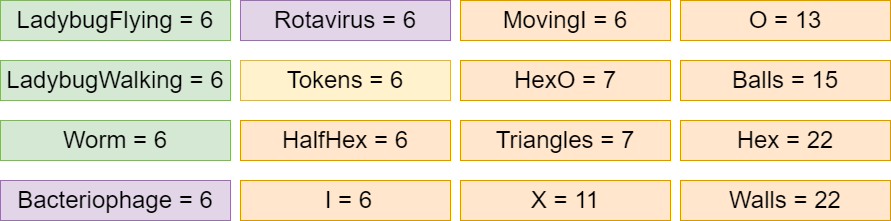
\includegraphics[width=0.8\textwidth]{rot_values}
    \caption{\texttt{rots} values used for each obstacle type}
    \label{fig:rot_values}
\end{figure}

However, for obstacles such as \texttt{Walls} and \texttt{Balls}, this method was not viable. The reason being that running \texttt{env=Balls} or \texttt{env=Walls} with visuals caused the game to lag significantly due to the number of animations playing simultaneously. As a result, \texttt{Walls} received the same number of rotations as \texttt{Hex} trap, while \texttt{Balls} received 15 rotations, the number at which the agent managed to learn. For bug, virus, and token obstacles, the default and minimum value of 6 rotations was assigned, with which they all trained successfully.
Concerning the \texttt{dists} parameter, it was concluded during the experiments that all agents could learn any obstacle with \texttt{dists=1}, and increasing this number needlessly would only increase the number of states required for training. 

After addressing the the issue of game not being playable, the most straightforward method for identifying the number of rotations required was to play the game manually with decreased speed. The results obtained from these experiments are displayed in Figure \ref{fig:rot_values} and were used in all experiments conducted. However, this method was not viable for obstacles such as \texttt{Walls} and \texttt{Balls} due to game lag. Thus, we assigned the same number of rotations to \texttt{Walls} as to the \textbf{Hex} trap, and to \texttt{Balls}, we assigned 15 rotations, the number at which the agent learned. \texttt{Bug}, \texttt{virus}, and \texttt{token} obstacles were assigned a default and minimum value of 6 rotations, which proved to be sufficient for successful training. During experiments, it was observed that all agents could learn any obstacle with \texttt{dists=1}, and increasing this parameter needlessly increased the number of required states.

The remaining values to be determined for the experiments were the suboptions for each agent (see \ref{opt:agent}). Even thought some of the experiments were omitted from this study, they provided useful insights that could be utilized. For instance, in many of those experiments, the agent performed best with \texttt{eps} values ranging from 0.2 to 0.4, with 0.2 being the most common, in combination with an \texttt{epsFinal} value of 0.0001. The rationale for using a low \texttt{epsFinal} value is that towards the end, the agent almost exclusively exploits the current policy, and a more gradual decrease in epsilon values is suitable for larger values of \texttt{n}. Furthermore, \texttt{initOptVal} of 20.0 and 100.0 was promising in most experiments. The \texttt{gam} value will be discussed in a later subsection.

Throughout the months dedicated to conducting experiments, they gradually converged towards checking combinations of the values mentioned above. Due to their length, the experiments and the number of parameters requiring adjustment, were kept systematic towards the end. Unless specified otherwise, each combination was tested on ten seeds for each agent, with the combinations consisting of \texttt{eps} parameter taking a value of either 0.2 or 0.4, and the \texttt{initOptVal} being either 20.0 or 100.0. Discounting was kept at the value of 1.0 (see Section \ref{intbeh}) and \texttt{epsFinal} was 0.0001.

Finally, it should mentioned how we shoose the number of games for an experiment. The general practice was to choose \texttt{n} 10 to 15 times greater than the number of obstacles the environment used for a particular experiment. This approach was found to be sufficient for facilitating the training of the agents. However, when incorporating the shooting actions, it was deemed appropriate to increase the value of \texttt{n} by approximately 25\%. Although this increase appeared reasonable, there was no specific rationale behind it.

\section{Interpreting the plots}
\label{plot_interpr}
\begin{figure}[h]
    \centering
    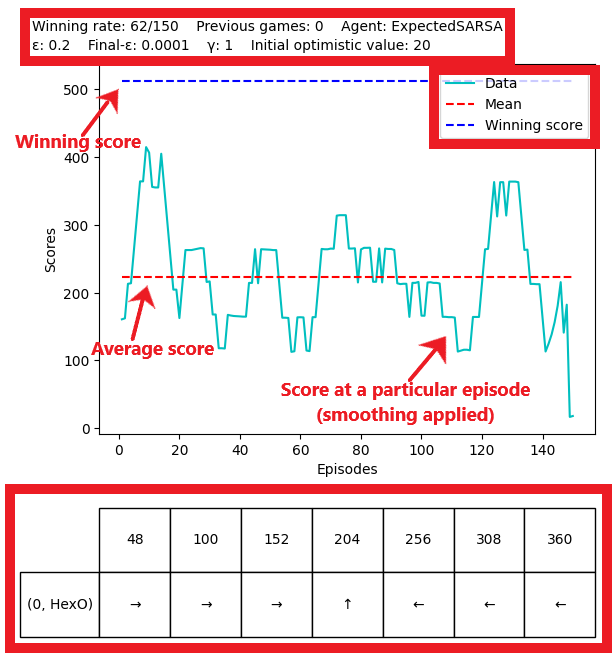
\includegraphics[width=0.7\textwidth]{examplePlot}
    \caption{Plot example}
    \label{fig:plt_eg}
\end{figure}

In Chapter \ref{experiments_chapter}, a number of plots similar to the one shown in Figure \ref{fig:plt_eg} will be presented. This section has been dedicated to explaining the different components of these plots and how to read them. While some plots may differ slightly from the one in Figure \ref{fig:plt_eg}, the meaning behind them can still be easily deduced.

The top part of the figure displays all the necessary information that was used in the experiment. Most of the values have been previously described, except for ``Previous games''. This value is meant for experiments that used the \texttt{database=read} option and were performed on an agent that had trained for some number of games. This number specifies the how many of games the agent had previously trained on.

Moving further down, there is a plot with three lines and a legend in the top right corner. The data line, as indicated on the figure, represents the score that the agent achieved on a particular episode. However, some plots may show the average value of the agent's score for each episode over several different seeds used for the random actions. Additionally, there may be multiple data lines on the plot, each averaged between many seeds and each representing a different agent. Every agent is labelled with their respective color inside the legend.

The mean line represents the average score value for the entire experiment, while the winning score represents the winning threshold which is the score that the agent achieves after passing level 15. This score will be constant (a little over 500), except in the cases where the environments contains any of the bugs and viruses and the agent is allowed to shoot. The winning score then depends on how many of those obstacles the agent successfully shoots. In this case the line will show the winning score of the last game in which the agent won. It should be noted that if the agent did not win any games, or the plot is displaying multiple agents, the winning score line will be omitted. Furthermore, the data line is averaged to appear smoother. This is why even though the winning rate is 62/150 in this sample plot, the data line doesn't touch the winning score threshold at any point.

As mentioned in Section \ref{commOpt}, it is possible to perform continuous evaluation on experiments, meaning one learning game is played with random actions, followed immediately by an evaluation game using only the current policy that the agent is performing. In all experiments conducted, the data line only represents the evaluation games.

At the very bottom of the figure, there is a table which only appears in plots that contain a single data line that is not averaged over different seeds and has only one seed value. In the table, all rotation values for this experiment define the columns, while each row has a tuple of distance value and type of the next obstacle ahead. Each cell then represents a particular discrete state, and the arrow it shows is the action that the agent takes in that state. If the arrow has \textit{*} attached to it, it means that the agent will also shoot. Since all experiments are performed with \texttt{dists=1}, the number of rows will match only the number of different obstacles used in the experiment.

It should be emphasized that parameters such as the number of seeds in the averaged data line or the size of the smoothing window will be clearly specified for each plot mentioned in the rest of the chapter. This prevents any form of ambiguity or confusion regarding the details of the experiment.

\section{Testing and plotting systems usage}
To produce the experiments and plots for this study, two scripts were written - one for conducting tests and the other for creating plots.  In this chapter, we provide a brief overview of how to use these scripts in case readers wish to replicate our experiments. Both scripts have an additional .txt file describing the process in more detail. Additionally, both of these systems produce a folder containing log files so that the user might see more closely what was happening during the run of either of the programs.

\subsection{Testing}
The \texttt{./test.py} script is designed to facilitate the running of multiple experiments at once, eliminating the need for users to manually run each experiment through the command line.

There are two types of variables: immutable and mutable. Immutable variables remain constant throughout all experiments, while mutable variables can be specified as a range of values. For each combination of mutable variables, the agent will run an experiment.

Immutable variables include \texttt{n, stoppingPoint, shooting, env, agent,} \\\texttt{ m, level, database, ceval,} and \texttt{debug}, which are defined in Section \ref{commOpt}. The variable \texttt{m} represents a range of \texttt{agentsSeed} values, with the default value of \texttt{m=[0,9]} (inclusive).

Mutable variables include sub-options for each agent, which are specified in the following format: \texttt{[min,max(not inclusive),step]}.

Additionally, there are top-level experiment options such as \texttt{all\_traps}, \\ \texttt{all\_bugs}, and \texttt{all\_viruses}, which run experiments for each individual trap, bug, or virus, respectively. There is also the option of \texttt{all\_agents}, which runs experiments with each learning agent, and \texttt{all\_shooting}, which runs experiments with both shooting on and off. These options overwrite equivalent immutable variables for \texttt{env}, \texttt{agent}, and \texttt{shooting}.

Note that the values for \texttt{rots} and \texttt{dists} for each \texttt{env} are hardcoded and cannot be changed.

Example usages are provided in the following code excerpts.

\begin{center}
\hrulefill
\begin{lstlisting}
# print description options
$ python ./test.py --description
\end{lstlisting}
\hrulefill
\end{center}
    
\begin{center}
\hrulefill
\begin{lstlisting}
# for 10 seeds run 100 full games with MonteCarlo agent
# perform continuous evaluation and write the output to the database
$ python ./test.py
\end{lstlisting}
\hrulefill
\end{center}
    
\begin{center}
\hrulefill
\begin{lstlisting}
# for each agent 5 times run 50 games on the environment with X trap
$ python ./test.py --m=[0,4] --n=50 --all_agents --env=[X]
\end{lstlisting}
\hrulefill
\end{center}

\begin{center}
\hrulefill
\begin{lstlisting}
# for 10 different seed values run 800 games for all combinations of:
# each of the DoubleQLearning and SARSA agents,
# on the Bugs environment with epsilon value 0.2
# and each of the initOpt values 20.0 and 100.0
$ python ./test.py --n=800 --agent=[DoubleQLearning,SARSA] --env=[Bugs] --eps=[0.2,0.3,0.1] --initOptVal=[20.0,180.0,80.0]
\end{lstlisting}
\hrulefill
\end{center}

\subsection{Plotting}

The \texttt{plots.py} script utilizes the files generated in the Command\_outputs folder to plot the outcomes of the experiments. The folder and its contents are automatically produced when the write option of the database is enabled. These files contain scores for each game in a single experiment, the resulting policy, and other relevant information that are displayed on the plots as described in Section \ref{plot_interpr} of this chapter.

Compared to the testing script, this system is much simpler as it only involves 2 parameters. The first parameter, \texttt{window}, has a default value of 10 and determines the number of neighboring points that will be averaged to produce smoother plots.

The second parameter is \texttt{option} whose value can be either 1 or 2. Option 1 generates 1 plot for each file in the Command\_outputs folder, while option 2 combines multiple files. In this case, for each distinct environment presented in the files, a single plot is created, with a data line for each agent averaged over multiple seeds. The number of seed values included and which agents are displayed depend solely on the accuracy of the files in the Command\_outputs folder.

Example usage is depicted in the command below.

\begin{center}
\hrulefill
\begin{lstlisting}
$ python ./plot.py --option=2 window=100
\end{lstlisting}
\hrulefill
\end{center}
